% Book 4, Year 2, chapter 23 -- Context-free grammars and pushdown automata.
% Provenance (never printed): sources/book4/BRIEFS.md, chapter 23.
\chapter{Context-Free Grammars and Pushdown Automata}\label{ch:b2:context-free-languages}

\Cref{ch:b2:regular-languages} proved that no finite automaton recognises the balanced bracket words, and so none
checks the brackets of an arithmetic expression or of a program. Two rules describe them all:

\omcode{code/bachelor-2/23-context-free-languages/listings/hook.rs}{17}{32}{A grammar of two rules, and every bracket
word up to length 10 tested against a counter}\label{lst:b2:context-free-languages:hook}

\omoutput{code/bachelor-2/23-context-free-languages/outputs/hook.txt}{The balanced words: 1, 1, 2, 5, 14, 42 of each
even length, and the grammar generates exactly them.}\label{out:b2:context-free-languages:hook}

The rule reads: a balanced word is empty, or an opening bracket, a balanced word, the closing bracket, and another
balanced word. A rule may name itself inside brackets, so the description nests to any depth, which a finite memory
cannot. This chapter defines such grammars, the trees they give to words and the trouble when a word has two, a normal
form and the cubic-time algorithm that decides membership for any grammar, the automata with a stack that recognise
the same languages, and the languages that are still out of reach.

\begin{recall}
\Cref{ch:b2:finite-automata,ch:b2:regular-languages}: words, languages, DFAs and NFAs, \omterm{def:b2:regular-languages:regex}{regular expressions}, the
pumping lemma for \omterm{def:b2:regular-languages:regular}{regular languages}, $\{a^nb^n\}$ not regular, closure of \omterm{def:b2:regular-languages:regular}{regular languages} under intersection. The
Year 1 volume: trees, their height, a binary tree of height $h$ has at most $2^h$ leaves; dynamic programming, filling a
table of answers to subproblems from the smallest up.
\end{recall}

\section{Grammars}\label{sec:b2:context-free-languages:grammars}

\begin{definition}[Context-free grammar]\label{def:b2:context-free-languages:grammar}
A \emph{context-free grammar}\index{context-free grammar} is $G = (N, \Sigma, P, S)$: a finite set $N$ of
\emph{nonterminals}\index{nonterminal}, an \omterm{def:b2:finite-automata:word}{alphabet} $\Sigma$ of \emph{terminals}\index{terminal (grammar)} disjoint
from $N$, a finite set $P$ of \emph{productions}\index{production (grammar)} $A \to \alpha$ with $A \in N$ and $\alpha
\in (N \cup \Sigma)^*$, and a \emph{start symbol}\index{start symbol} $S \in N$. Productions with the same left side
are written together, $A \to \alpha \mid \beta$.
\end{definition}

\begin{definition}[Derivation, generated language]\label{def:b2:context-free-languages:derivation}
A word over $N \cup \Sigma$ is a \emph{sentential form}. If $A \to \alpha$ is a production, $\beta A \gamma \Rightarrow
\beta \alpha \gamma$ is an \emph{immediate derivation}; a \emph{derivation}\index{derivation (grammar)} $\alpha
\Rightarrow^* \beta$ is a sequence of zero or more of them. The language \emph{generated}\index{generated language}
by $G$ is $L(G) = \{w \in \Sigma^* : S \Rightarrow^* w\}$. A language is
\emph{context-free}\index{context-free language} if some \omterm{def:b2:context-free-languages:grammar}{context-free grammar} generates it.
\end{definition}

``\omterm{def:b2:context-free-languages:derivation}{Context-free}'' says that a \omterm{def:b2:context-free-languages:grammar}{nonterminal} is replaced whatever surrounds it. The listings write a grammar one
\omterm{def:b2:context-free-languages:grammar}{nonterminal} per line, a name with a capital for a \omterm{def:b2:context-free-languages:grammar}{nonterminal}, one character for a terminal, and \code{ε} for the empty
right side; the library \code{grammar.rs} reads that text. Three grammars of familiar languages:
\begin{itemize}
\item arithmetic expressions: $E \to E + E \mid E * E \mid (E) \mid a$, with $a$ standing for any number or name;
\item propositional formulas over the variables $p$, $q$: $F \to F \vee F \mid F \wedge F \mid \neg F \mid (F) \mid p
\mid q$;
\item a toy markup, where $w$ is a word, $[\,\cdots]$ a link and $*\cdots*$ bold text: $D \to D\,D \mid w \mid *D* \mid
[D]$.
\end{itemize}
The \omterm{def:b2:context-free-languages:derivation}{derivations} of $()()$ from $S \to (S)S \mid \varepsilon$ include $S \Rightarrow (S)S \Rightarrow ()S \Rightarrow
()(S)S \Rightarrow ()()S \Rightarrow ()()$. Which words a grammar generates is computed by
\code{generated}, a fixed point: start with nothing, and add to each \omterm{def:b2:context-free-languages:grammar}{nonterminal} the concatenations of what the
symbols of its right sides already derive, cut at a length $n$, until nothing changes.

\begin{definition}[Right-linear grammar]\label{def:b2:context-free-languages:right-linear}
A grammar is \emph{right-linear}\index{right-linear grammar} if every production is $A \to uB$ or $A \to u$, with $u
\in \Sigma^*$ and $B \in N$: a \omterm{def:b2:context-free-languages:grammar}{nonterminal}, if any, comes last.
\end{definition}

\begin{proposition}[Regular languages are context-free]\label{prop:b2:context-free-languages:right-linear}
A language is regular if and only if a \omterm{def:b2:context-free-languages:right-linear}{right-linear grammar} generates it. So every \omterm{def:b2:regular-languages:regular}{regular language} is \omterm{def:b2:context-free-languages:derivation}{context-free},
and $\{a^nb^n : n \ge 0\}$, \omterm{def:b2:context-free-languages:derivation}{generated} by $S \to aSb \mid \varepsilon$, shows the inclusion is strict.
\end{proposition}

\begin{proof}
From a DFA, take one \omterm{def:b2:context-free-languages:grammar}{nonterminal} per state, the start state as \omterm{def:b2:context-free-languages:grammar}{start symbol}, a production $q \to a\,\delta(q, a)$ per
transition and $q \to \varepsilon$ per \omterm{def:b2:finite-automata:dfa}{accepting state}: a \omterm{def:b2:context-free-languages:derivation}{derivation} $q_0 \Rightarrow a_1 q_1 \Rightarrow a_1 a_2 q_2
\Rightarrow \cdots$ follows a run, and ends in a word exactly when the run ends in an \omterm{def:b2:finite-automata:dfa}{accepting state}. Conversely,
cut each production $A \to a_1 \cdots a_k B$ into a chain of $k$ transitions through $k - 1$ new states, from state $A$
to state $B$ (a spontaneous one if $k = 0$), and each $A \to a_1 \cdots a_k$ into a chain to one new \omterm{def:b2:finite-automata:dfa}{accepting state}:
the NFA's runs follow the \omterm{def:b2:context-free-languages:derivation}{derivations}, and \cref{ch:b2:finite-automata} makes it deterministic.
\end{proof}

\section{Parse trees and ambiguity}\label{sec:b2:context-free-languages:trees}

\begin{definition}[Parse tree, leftmost and rightmost derivation]\label{def:b2:context-free-languages:parse-tree}
A \emph{parse tree}\index{parse tree} for $G$ is an ordered tree whose root is $S$, whose inner nodes are \omterm{def:b2:context-free-languages:grammar}{nonterminals},
whose leaves are \omterm{def:b2:context-free-languages:grammar}{terminals} or $\varepsilon$, and where the children of each inner node $A$, read from left to right,
are the right side of a production $A \to \alpha$. Its \emph{yield} is its leaves read from left to right. A
\omterm{def:b2:context-free-languages:derivation}{derivation} is \emph{leftmost}\index{leftmost derivation} if each step replaces the leftmost \omterm{def:b2:context-free-languages:grammar}{nonterminal}, and
\emph{rightmost}\index{rightmost derivation} if each replaces the rightmost one.
\end{definition}

A word is in $L(G)$ exactly when it is the yield of a \omterm{def:b2:context-free-languages:parse-tree}{parse tree}, and \omterm{def:b2:context-free-languages:parse-tree}{parse trees}, \omterm{def:b2:context-free-languages:parse-tree}{leftmost derivations} and \omterm{def:b2:context-free-languages:parse-tree}{rightmost
derivations} of a word are in bijection: a tree is turned into its \omterm{def:b2:context-free-languages:parse-tree}{leftmost derivation} by expanding its nodes in
preorder, and a \omterm{def:b2:context-free-languages:derivation}{derivation} into a tree by hanging each production's right side under the node it expands. The method
\code{leftmost} finds a \omterm{def:b2:context-free-languages:parse-tree}{leftmost derivation} by a breadth-first search over sentential forms, dropping those whose
first \omterm{def:b2:context-free-languages:grammar}{terminals} do not match the word:

\omoutput{code/bachelor-2/23-context-free-languages/outputs/derive.txt}{A grammar of expressions with one \omterm{def:b2:context-free-languages:grammar}{nonterminal}
per level of priority, and the \omterm{def:b2:context-free-languages:parse-tree}{leftmost derivation} of $a + a * a$.}\label{out:b2:context-free-languages:derive}

\begin{definition}[Ambiguous grammar, weak equivalence]\label{def:b2:context-free-languages:ambiguous}
A grammar is \emph{ambiguous}\index{ambiguous grammar} if some word has two different \omterm{def:b2:context-free-languages:parse-tree}{parse trees}. Two grammars are
\emph{weakly equivalent}\index{weak equivalence (grammars)} if they generate the same language, whatever trees they
give.
\end{definition}

A program reads meaning from the tree. In the grammar $E \to E + E \mid E * E \mid (E) \mid a$, $a + a * a$ has a tree
that multiplies first and one that adds first, two different values:

\begin{omfigure}
\begin{forest}
for tree={font=\small, l sep=6pt, s sep=8pt}
[$E$ [$E$ [$a$]] [$+$] [$E$ [$E$ [$a$]] [$*$] [$E$ [$a$]]]]
\end{forest}
\hspace{2cm}
\begin{forest}
for tree={font=\small, l sep=6pt, s sep=8pt}
[$E$ [$E$ [$E$ [$a$]] [$+$] [$E$ [$a$]]] [$*$] [$E$ [$a$]]]
\end{forest}
\par\smallskip{\small Two \omterm{def:b2:context-free-languages:parse-tree}{parse trees} of $a + a * a$ in the grammar $E \to E + E \mid E * E \mid (E) \mid a$. Left:
$a + (a * a)$; right: $(a + a) * a$.}
\end{omfigure}

The grammar of \cref{out:b2:context-free-languages:derive} removes the ambiguity with one \omterm{def:b2:context-free-languages:grammar}{nonterminal} per level: an
expression $E$ is a sum of terms $T$, a term a product of factors $F$, and a factor a letter or a bracketed expression.
A $+$ can then appear inside a product only within brackets, so multiplication binds tighter; and since $E \to E + T$
has its recursion on the left, $a + a + a$ groups as $(a + a) + a$. The function \code{trees} of \code{count.rs} counts
\omterm{def:b2:context-free-languages:parse-tree}{parse trees} by dynamic programming over the spans of the word:

\omoutput{code/bachelor-2/23-context-free-languages/outputs/ambiguity.txt}{\omterm{def:b2:context-free-languages:parse-tree}{Parse trees} counted in the flat and the
levelled expression grammars, then in two grammars of
\code{if}\ldots\code{else}.}\label{out:b2:context-free-languages:ambiguity}

The two expression grammars are \omterm{def:b2:context-free-languages:ambiguous}{weakly equivalent}, as the program checks up to length 7. The second pair is the
\emph{dangling else}: with $i$ for ``if a condition then'', $e$ for ``else'' and $x$ for any other statement, $S \to iS
\mid iSeS \mid x$ gives $iixex$ two trees, the \code{else} belonging to either \code{if}.

\begin{omfigure}
\begin{forest}
for tree={font=\small, l sep=6pt, s sep=8pt}
[$S$ [$i$] [$S$ [$i$] [$S$ [$x$]] [$e$] [$S$ [$x$]]]]
\end{forest}
\hspace{2cm}
\begin{forest}
for tree={font=\small, l sep=6pt, s sep=8pt}
[$S$ [$i$] [$S$ [$i$] [$S$ [$x$]]] [$e$] [$S$ [$x$]]]
\end{forest}
\par\smallskip{\small The dangling \code{else}: in $iixex$, the \code{else} belongs to the inner \code{if} (left) or to
the outer one (right).}
\end{omfigure}

Languages settle it by a rule, ``an \code{else} belongs to the nearest \code{if} without one'', and the grammar
$S \to M \mid U$, $M \to iMeM \mid x$, $U \to iS \mid iMeU$ writes the rule down: between an $i$ and its $e$ only a
\emph{matched} statement $M$, every $i$ of which has its $e$, may appear. It is \omterm{def:b2:context-free-languages:ambiguous}{weakly equivalent} to the first and
unambiguous on every word the program tried. Some \omterm{def:b2:context-free-languages:derivation}{context-free languages} have no unambiguous grammar at all, and no
program can decide in general whether a grammar is \omterm{def:b2:context-free-languages:ambiguous}{ambiguous}; these facts are proved in more advanced texts.

\section{Chomsky normal form}\label{sec:b2:context-free-languages:cnf}

\begin{definition}[Chomsky normal form]\label{def:b2:context-free-languages:cnf}
A grammar is in \emph{Chomsky normal form}\index{Chomsky normal form} if every production is $A \to BC$ with $B, C$
\omterm{def:b2:context-free-languages:grammar}{nonterminals}, or $A \to a$ with $a$ a terminal, except possibly $S \to \varepsilon$ when the \omterm{def:b2:context-free-languages:grammar}{start symbol} $S$ appears in
no right side. Its \emph{size} $|G|$ is the sum over the \omterm{def:b2:context-free-languages:grammar}{productions} of one plus the length of the right side.
\end{definition}

\begin{method}[Conversion to Chomsky normal form]\label{met:b2:context-free-languages:cnf}
Apply in this order:
\begin{enumerate}
\item START: if $S$ derives $\varepsilon$ and appears in a right side, add a new start $S_0 \to S$;
\item TERM: in every right side of length at least 2, replace each terminal $c$ by a new \omterm{def:b2:context-free-languages:grammar}{nonterminal} written
\code{'c'}, with \code{'c'} $\to c$;
\item BIN: cut every $A \to X_1 X_2 \cdots X_k$ with $k \ge 3$ into $A \to X_1 Y_1$, $Y_1 \to X_2 Y_2$, \dots, $Y_{k-2}
\to X_{k-1} X_k$, with new \omterm{def:b2:context-free-languages:grammar}{nonterminals} $Y_i$;
\item DEL: compute the nullable \omterm{def:b2:context-free-languages:grammar}{nonterminals} (those that derive $\varepsilon$); for every production, add each version
with some nullable occurrences dropped; then remove every $A \to \varepsilon$ except $S \to \varepsilon$;
\item UNIT: for each $A$, find by a graph search the \omterm{def:b2:context-free-languages:grammar}{nonterminals} $B$ with $A \Rightarrow^* B$ through \omterm{def:b2:context-free-languages:grammar}{productions} with
one \omterm{def:b2:context-free-languages:grammar}{nonterminal} on the right; give $A$ every non-unit production of each such $B$; remove the unit \omterm{def:b2:context-free-languages:grammar}{productions}.
\end{enumerate}
\end{method}

\omcode{code/bachelor-2/23-context-free-languages/listings/grammar.rs}{166}{200}{START, TERM and BIN: new names for
the \omterm{def:b2:context-free-languages:grammar}{terminals} and for the pieces of long right sides}\label{lst:b2:context-free-languages:cnf1}

\omcode{code/bachelor-2/23-context-free-languages/listings/grammar.rs}{201}{238}{DEL and UNIT: every way to drop
nullable symbols, then every production reachable through unit chains}\label{lst:b2:context-free-languages:cnf2}

\begin{proposition}[The normal form]\label{prop:b2:context-free-languages:cnf}
The method returns a grammar in \omterm{def:b2:context-free-languages:cnf}{Chomsky normal form} that generates $L(G)$, of size at most proportional to $|G|^2$.
\end{proposition}

\begin{proof}
START, TERM and BIN keep the language: each new \omterm{def:b2:context-free-languages:grammar}{nonterminal} derives exactly the piece it replaces. DEL: if a version
drops nullable symbols, the dropped symbols could derive $\varepsilon$ in $G$, so nothing new is \omterm{def:b2:context-free-languages:derivation}{generated}; conversely,
in a \omterm{def:b2:context-free-languages:parse-tree}{parse tree} of a nonempty word, cutting every subtree whose yield is empty leaves a tree that uses only the new
versions. UNIT: a chain of unit \omterm{def:b2:context-free-languages:grammar}{productions} $A \Rightarrow B \Rightarrow \cdots \Rightarrow C \Rightarrow \alpha$ in a
\omterm{def:b2:context-free-languages:derivation}{derivation} is replaced by the one production $A \to \alpha$, and every new production stands for such a chain; the
search stops on a cycle of unit \omterm{def:b2:context-free-languages:grammar}{productions} because it visits each \omterm{def:b2:context-free-languages:grammar}{nonterminal} once. After BIN every right side has
at most two symbols, so DEL makes at most three versions of each production, and the size stays proportional to $|G|$
up to that point. UNIT gives each of at most $|G|$ \omterm{def:b2:context-free-languages:grammar}{nonterminals} a copy of at most all the \omterm{def:b2:context-free-languages:grammar}{productions}: at most
$|G|^2$.
\end{proof}

The order matters: DEL before BIN would make $2^k$ versions of a right side with $k$ nullable symbols. The expression
grammar with levels has no $\varepsilon$ and so needs no new start:

\omoutput{code/bachelor-2/23-context-free-languages/outputs/cnf.txt}{The expression grammar in \omterm{def:b2:context-free-languages:cnf}{Chomsky normal form},
and a check of its words.}\label{out:b2:context-free-languages:cnf}

The unit \omterm{def:b2:context-free-languages:grammar}{productions} $E \to T$ and $T \to F$ are gone: $E$ now has the \omterm{def:b2:context-free-languages:grammar}{productions} of $T$ and $F$ as well.

\section{The CYK algorithm}\label{sec:b2:context-free-languages:cyk}

In \omterm{def:b2:context-free-languages:cnf}{Chomsky normal form}, a \omterm{def:b2:context-free-languages:grammar}{nonterminal} derives a word of length at least 2 by splitting it into two nonempty parts,
derived by the two \omterm{def:b2:context-free-languages:grammar}{nonterminals} of a production. A table over the factors of the word, filled from the shortest up,
decides membership.

\begin{method}[The CYK algorithm]\label{met:b2:context-free-languages:cyk}
Let $G$ be in \omterm{def:b2:context-free-languages:cnf}{Chomsky normal form} and $w = a_1 \cdots a_n$ nonempty. For the factor of length $\ell$ starting after
position $i$, compute the set $T[i][\ell]$ of \omterm{def:b2:context-free-languages:grammar}{nonterminals} that derive it: $T[i][1] = \{A : A \to a_{i+1}\}$, and for
$\ell = 2, \dots, n$, $T[i][\ell]$ holds $A$ whenever there are a production $A \to BC$ and a split $1 \le k < \ell$
with $B \in T[i][k]$ and $C \in T[i + k][\ell - k]$. Then $w \in L(G)$ if and only if $S \in
T[0][n]$.\index{CYK algorithm}
\end{method}

\omcode{code/bachelor-2/23-context-free-languages/listings/grammar.rs}{270}{300}{CYK: the table, one cell per factor,
and a count of the split points}\label{lst:b2:context-free-languages:cyk}

\omoutput{code/bachelor-2/23-context-free-languages/outputs/cyk.txt}{The table of $a + a * a$, the whole word on top,
the letters at the bottom.}\label{out:b2:context-free-languages:cyk}

\begin{omfigure}
\begin{tikzpicture}[x=1.6cm, y=0.75cm, font=\scriptsize]
\foreach \len/\row in {1/{{E,F,T},{\textquotesingle+\textquotesingle},{E,F,T},{\textquotesingle*\textquotesingle},{E,F,T}},
    2/{{},{X0},{},{X1}}, 3/{{E},{},{E,T}}, 4/{{},{X0}}, 5/{{E}}} {
  \foreach \cell [count=\i from 0] in \row {
    \draw[omDef!60] (\i + 0.5*\len - 0.5, \len) rectangle ++(1, 0.8);
    \node at (\i + 0.5*\len, \len + 0.4) {\texttt{\{\cell\}}};
  }
}
\foreach \c [count=\i from 0] in {a, +, a, *, a} \node at (\i + 0.5, 0.4) {\small $\c$};
\end{tikzpicture}
\par\smallskip{\small The CYK table of $a + a * a$ as a pyramid: each cell sits above the factor it covers. The top
cell holds $E$, so the word is an expression; the cell over $a + a$ holds $E$, and the one over $a * a$ holds $E$ and
$T$.}
\end{omfigure}

\begin{theorem}[CYK]\label{thm:b2:context-free-languages:cyk}
The \omterm{met:b2:context-free-languages:cyk}{CYK algorithm} decides whether $w \in L(G)$. It examines $(n^3 - n)/6$ split points, each against every production
$A \to BC$, so its time is proportional to $n^3 |G|$.
\end{theorem}

\begin{proof}
By induction on $\ell$, $A \in T[i][\ell]$ if and only if $A \Rightarrow^* a_{i+1} \cdots a_{i+\ell}$. For $\ell = 1$,
in \omterm{def:b2:context-free-languages:cnf}{Chomsky normal form} a \omterm{def:b2:context-free-languages:grammar}{nonterminal} derives a letter only through a production $A \to a$. For $\ell \ge 2$, a
\omterm{def:b2:context-free-languages:derivation}{derivation} of the factor starts with some $A \to BC$, and $B$ and $C$ then derive a nonempty prefix of length $k$ and
the rest, which by the hypothesis is when $B \in T[i][k]$ and $C \in T[i + k][\ell - k]$. For the count: a factor of
length $\ell$ has $\ell - 1$ split points, and there are $n - \ell + 1$ factors of that length, so the number of
split points is
\[
\sum_{\ell=2}^{n} (n - \ell + 1)(\ell - 1) = \sum_{j=1}^{n-1} (n - j)j = n \frac{(n - 1)n}{2} - \frac{(n - 1)n(2n -
1)}{6} = \frac{n^3 - n}{6}.
\]
\end{proof}

The table holds more than a yes or no. Replacing each set by a count of trees per \omterm{def:b2:context-free-languages:grammar}{nonterminal}, a product for each
split and a sum over splits and \omterm{def:b2:context-free-languages:grammar}{productions}, counts the \omterm{def:b2:context-free-languages:parse-tree}{parse trees} of the word. For $E \to E + E \mid a$ on $a + a +
\cdots + a$ with $k$ operands, a tree chooses the $+$ at its root and then trees for both sides, the recurrence of the
Catalan numbers, $C_{k-1} = \frac{1}{k}\binom{2k - 2}{k - 1}$:

\omoutput{code/bachelor-2/23-context-free-languages/outputs/count_trees.txt}{\omterm{def:b2:context-free-languages:parse-tree}{Parse trees} of a sum of $k$ operands in
the \omterm{def:b2:context-free-languages:ambiguous}{ambiguous grammar}, against the Catalan numbers.}\label{out:b2:context-free-languages:catalan}

One \omterm{def:b2:context-free-languages:ambiguous}{ambiguous} rule gives a sum of 20 operands 1\,767\,263\,190 trees; from 38 operands the count no longer fits in
64 bits (\cref{exo:b2:context-free-languages:11}).

\begin{history}
% ledger: b2:chomsky-1956
% ledger: b2:algol60-report
% ledger: b2:younger-1967
Noam Chomsky described phrase-structure grammars, the \omterm{def:b2:context-free-languages:derivation}{context-free} ones among them, in a paper of 1956 on models of
language. Programming languages took them up at once: the report on ALGOL 60, edited by Peter Naur in 1960, gave the
language's syntax as a grammar in a notation since called Backus--Naur form. The cubic algorithm carries the initials
of John Cocke, Daniel Younger and Tadao Kasami, who found it independently in the 1960s; Younger's paper appeared in
1967.
\end{history}

\section{Pushdown automata}\label{sec:b2:context-free-languages:pda}

A finite automaton cannot count; give it a stack and it can.

\begin{definition}[Pushdown automaton]\label{def:b2:context-free-languages:pda}
A \emph{pushdown automaton}\index{pushdown automaton} (PDA) is $(Q, \Sigma, \Gamma, \Delta, q_0, Z_0, F)$: a finite
set of states $Q$, an input \omterm{def:b2:finite-automata:word}{alphabet} $\Sigma$, a \emph{stack alphabet}\index{stack alphabet} $\Gamma$, a finite set
$\Delta$ of \emph{moves} $(q, x, Z) \to (q', \gamma)$ with $x \in \Sigma \cup \{\varepsilon\}$, $Z \in \Gamma$ and
$\gamma \in \Gamma^*$, a start state $q_0$, a bottom symbol $Z_0 \in \Gamma$, and \omterm{def:b2:finite-automata:dfa}{accepting states} $F \subseteq Q$. In
state $q$ with $Z$ on top of the stack, the move reads $x$ (nothing if $x = \varepsilon$), goes to $q'$ and replaces
$Z$ by $\gamma$, whose first symbol ends on top. A \emph{configuration} is a state, the unread input and the stack. The
automaton \emph{accepts} $w$ if some sequence of moves leads from $(q_0, w, Z_0)$ to a configuration with no input
left and an \omterm{def:b2:finite-automata:dfa}{accepting state}.
\end{definition}

\begin{omfigure}
\begin{tikzpicture}[->, >={Stealth[length=1.8mm]}, every state/.style={minimum size=7mm, inner sep=0pt},
    font=\scriptsize, auto, node distance=40mm]
\node[state, initial, initial text=] (0) {0};
\node[state] (1) [right of=0] {1};
\node[state, accepting] (2) [right of=1] {2};
\path (0) edge[loop above] node[align=center] {$a, Z / AZ$\\ $a, A / AA$} ()
  (0) edge node[align=center] {$\varepsilon, Z / Z$\\ $\varepsilon, A / A$} (1)
  (1) edge[loop above] node {$b, A / \varepsilon$} ()
  (1) edge node {$\varepsilon, Z / Z$} (2);
\end{tikzpicture}
\par\smallskip{\small A PDA for $\{a^nb^n\}$. A label $x, Z / \gamma$ reads $x$ with $Z$ on top and replaces it by
$\gamma$. State 0 pushes an $A$ per $a$; the move to 1 guesses the middle; state 1 pops an $A$ per $b$; state 2 is
reached when only the bottom $Z$ is left.}
\end{omfigure}

Like an NFA, a PDA may have several moves from one configuration. The listing explores the configurations by a search,
with a bound on the stack's height so that it always stops:

\omcode{code/bachelor-2/23-context-free-languages/listings/pda.rs}{23}{50}{Some run accepts: a search over
configurations}\label{lst:b2:context-free-languages:pda}

\omoutput{code/bachelor-2/23-context-free-languages/outputs/pda_demo.txt}{The automaton above, and the automaton built
from $S \to (S)S \mid \varepsilon$ by \cref{thm:b2:context-free-languages:cfg-to-pda}.}\label{out:b2:context-free-languages:pda}

\begin{theorem}[From a grammar to a pushdown automaton]\label{thm:b2:context-free-languages:cfg-to-pda}
For every \omterm{def:b2:context-free-languages:grammar}{context-free grammar} $G$ there is a PDA with three states that recognises $L(G)$.
\end{theorem}

\begin{proof}
\omterm{def:b2:context-free-languages:pda}{Stack alphabet} $N \cup \Sigma \cup \{\$\}$, states 0, 1, 2, accepting 2. Moves: $(0, \varepsilon, \$) \to (1, S\$)$;
for each production $A \to \alpha$, $(1, \varepsilon, A) \to (1, \alpha)$; for each terminal $a$, $(1, a, a) \to (1,
\varepsilon)$; and $(1, \varepsilon, \$) \to (2, \varepsilon)$. The claim, by induction on the number of steps: in
state 1, the automaton can go from $(1, xy, S\$)$ to $(1, y, \alpha\$)$ exactly when there is a \omterm{def:b2:context-free-languages:parse-tree}{leftmost derivation} $S
\Rightarrow^* x\alpha$ with $x$ the \omterm{def:b2:context-free-languages:grammar}{terminals} already matched and $\alpha$ empty or starting with a \omterm{def:b2:context-free-languages:grammar}{nonterminal} (or,
between two steps, with a terminal still to match). An expansion move is a step of the \omterm{def:b2:context-free-languages:derivation}{derivation}; a matching move
reads a letter that the \omterm{def:b2:context-free-languages:derivation}{derivation} has already produced. So the automaton reaches $(1, \varepsilon, \$)$, and then
state 2, exactly when $S \Rightarrow^* w$.
\end{proof}

\begin{theorem}[From a pushdown automaton to a grammar]\label{thm:b2:context-free-languages:pda-to-cfg}
For every PDA there is a \omterm{def:b2:context-free-languages:grammar}{context-free grammar} that generates the language it recognises. So the \omterm{def:b2:context-free-languages:derivation}{context-free languages}
are exactly the languages recognised by pushdown automata.
\end{theorem}

\admitted

The proof builds a \omterm{def:b2:context-free-languages:grammar}{nonterminal} for each pair of states and each stack symbol, deriving the words that lead from the
first state to the second while that symbol is popped. It is long and is not needed here. Deterministic automata are
another matter: the PDA for $\{a^nb^n\}$ guesses the middle, though a deterministic one exists (the first $b$ marks it); some
languages, such as the even-length palindromes,
need guessing, and the parsers of the Year 3 volume's chapters on parsing build deterministic PDAs from grammars of a
restricted kind.

\section{The limits of context-free languages}\label{sec:b2:context-free-languages:limits}

\begin{theorem}[Pumping lemma for context-free languages]\label{thm:b2:context-free-languages:pumping}
If $L$ is \omterm{def:b2:context-free-languages:derivation}{context-free}, there is $p$ such that every $z \in L$ with $|z| \ge p$ can be written $z = uvwxy$ with $|vwx|
\le p$ and $vx \ne \varepsilon$, so that $uv^iwx^iy \in L$ for every $i \ge 0$.
\end{theorem}

\begin{proof}
Take a grammar for $L$ in \omterm{def:b2:context-free-languages:cnf}{Chomsky normal form}, with $k$ \omterm{def:b2:context-free-languages:grammar}{nonterminals}, and $p = 2^k$. A \omterm{def:b2:context-free-languages:parse-tree}{parse tree} in this form is
binary above its leaves: if its longest path from the root to a terminal has $h$ \omterm{def:b2:context-free-languages:grammar}{nonterminals}, the word has at most
$2^{h-1}$ letters. So for $|z| \ge 2^k$ the tree has a path with at least $k + 1$ \omterm{def:b2:context-free-languages:grammar}{nonterminals}, and among the lowest
$k + 1$ of them some $A$ appears twice. Let the upper $A$ derive $vwx$ and the lower $A$ derive $w$, and $z = uvwxy$.
The subtree of the upper $A$ has paths of at most $k + 1$ \omterm{def:b2:context-free-languages:grammar}{nonterminals}, so $|vwx| \le 2^k = p$. The upper $A$ has two
children, the lower $A$ lies under one of them, and the other derives a nonempty word that is part of $v$ or $x$: $vx
\ne \varepsilon$. Replacing the lower subtree by a copy of the upper one, $i - 1$ times, or the upper by the lower,
gives trees of $uv^iwx^iy$.
\end{proof}

\begin{omfigure}
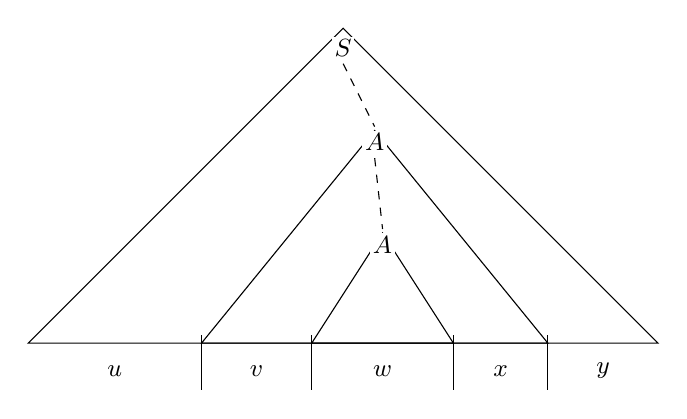
\begin{tikzpicture}[font=\small]
\draw (0, 0) -- (-4, -4) -- (4, -4) -- cycle;
\draw (0.4, -1.3) -- (-1.8, -4) -- (2.6, -4) -- cycle;
\draw (0.5, -2.6) -- (-0.4, -4) -- (1.4, -4) -- cycle;
\node[fill=white, inner sep=1pt] at (0, -0.25) {$S$};
\node[fill=white, inner sep=1pt] at (0.4, -1.45) {$A$};
\node[fill=white, inner sep=1pt] at (0.5, -2.75) {$A$};
\draw[dashed] (0, -0.45) -- (0.4, -1.25) (0.4, -1.65) -- (0.5, -2.55);
\foreach \x/\t in {-2.9/u, -1.1/v, 0.5/w, 2.0/x, 3.3/y} \node at (\x, -4.35) {$\t$};
\foreach \x in {-1.8, -0.4, 1.4, 2.6} \draw (\x, -3.9) -- (\x, -4.6);
\end{tikzpicture}
\par\smallskip{\small A long word has a tall tree, and a tall path repeats a \omterm{def:b2:context-free-languages:grammar}{nonterminal} $A$. The upper $A$ derives
$vwx$, the lower one $w$; either subtree can stand in for the other, which pumps $v$ and $x$
together.}
\end{omfigure}

\begin{proposition}[Closure]\label{prop:b2:context-free-languages:closure}
\omterm{def:b2:context-free-languages:derivation}{Context-free languages} are closed under union, concatenation and star, and under intersection with a \omterm{def:b2:regular-languages:regular}{regular
language}. They are not closed under intersection or complement. The language $\{a^nb^nc^n : n \ge 0\}$ is not
\omterm{def:b2:context-free-languages:derivation}{context-free}.
\end{proposition}

\begin{proof}
With \omterm{def:b2:context-free-languages:grammar}{start symbols} $S_1$, $S_2$ and disjoint \omterm{def:b2:context-free-languages:grammar}{nonterminals}, $S \to S_1 \mid S_2$, $S \to S_1 S_2$ and $S \to S_1 S \mid
\varepsilon$ give the union, the concatenation and the star. Intersection with a \omterm{def:b2:regular-languages:regular}{regular language} is
\cref{exo:b2:context-free-languages:12}. For $\{a^nb^nc^n\}$, take $z = a^pb^pc^p$: since $|vwx| \le p$, $vwx$ meets
at most two of the three blocks, so pumping with $i = 2$ changes the number of at most two of the letters (or breaks
their order) and leaves the word outside the language. Now $\{a^nb^nc^m\}$ and $\{a^mb^nc^n\}$ are \omterm{def:b2:context-free-languages:derivation}{context-free}, by
$S \to TC$, $T \to aTb \mid \varepsilon$, $C \to cC \mid \varepsilon$ and a symmetric grammar, and their intersection
is $\{a^nb^nc^n\}$: no closure under intersection. Since $L \cap M$ is the complement of the union of the complements,
closure under complement would give closure under intersection.
\end{proof}

A \omterm{def:b2:context-free-languages:pda}{pushdown automaton} has one stack, and $a^nb^nc^n$ needs to count twice. The same argument, applied after an
intersection with $a^+b^+a^+b^+$, shows that $\{ww\}$ is not \omterm{def:b2:context-free-languages:derivation}{context-free} either (\cref{exo:b2:context-free-languages:10}):
checking that two parts of a program agree, such as a variable's declaration and its uses, is beyond any grammar, and
compilers check it in a later pass with a table of names.

\section{Exercises}\label{sec:b2:context-free-languages:exercises}

\begin{exercise}[$\star$]\label{exo:b2:context-free-languages:1}
Give a \omterm{def:b2:context-free-languages:parse-tree}{leftmost derivation} of $(a) * a$ in the grammar with levels of \cref{out:b2:context-free-languages:derive}, and
draw its \omterm{def:b2:context-free-languages:parse-tree}{parse tree}.
\end{exercise}

\begin{exercise}[$\star$]\label{exo:b2:context-free-languages:2}
Someone writes $S \to (S)S \mid )S(S \mid \varepsilon$ for the balanced bracket words. Show that it generates $())($.
Which language does it generate?
\end{exercise}

\begin{exercise}[$\star$]\label{exo:b2:context-free-languages:3}
Write a grammar for the palindromes over $\{a, b\}$, and check it on every word of length at most 12.
\end{exercise}

\begin{exercise}[$\star$]\label{exo:b2:context-free-languages:4}
Draw the \omterm{def:b2:context-free-languages:parse-tree}{parse trees} of $a + a + a + a$ in $E \to E + E \mid E * E \mid (E) \mid a$. How many are there, and how many
does the grammar with levels give?
\end{exercise}

\begin{exercise}[$\star\star$]\label{exo:b2:context-free-languages:5}
For $S \to AB \mid AC$, $C \to SB$, $A \to a$, $B \to b$, fill the CYK tables of $aabb$ and $abab$. Which language does
the grammar generate?
\end{exercise}

\begin{exercise}[$\star\star$]\label{exo:b2:context-free-languages:6}
A program removes unit \omterm{def:b2:context-free-languages:grammar}{productions} by following them recursively from each \omterm{def:b2:context-free-languages:grammar}{nonterminal}. What happens on $S \to A \mid
ab$, $A \to B \mid a$, $B \to A \mid b$? How does \cref{met:b2:context-free-languages:cnf} avoid it, and what does it
produce?
\end{exercise}

\begin{exercise}[$\star\star$]\label{exo:b2:context-free-languages:7}
Write a recogniser for $S \to TS \mid c$, $T \to aSb$ with one function per \omterm{def:b2:context-free-languages:grammar}{nonterminal}, each reading one word of its
\omterm{def:b2:context-free-languages:grammar}{nonterminal} from the current position; the next letter tells which production to use. Check it against the grammar on
every word of length at most 9 over $\{a, b, c\}$.
\end{exercise}

\begin{exercise}[$\star\star$]\label{exo:b2:context-free-languages:8}
Prove that $S \to (S)S \mid \varepsilon$ generates exactly the balanced words: those with as many $($ as $)$ in which
no prefix has more $)$ than $($.
\end{exercise}

\begin{exercise}[$\star\star$]\label{exo:b2:context-free-languages:9}
Build a PDA for the words over $\{a, b\}$ with as many $a$ as $b$, and test it on all words of length at most 10.
\end{exercise}

\begin{exercise}[$\star\star\star$]\label{exo:b2:context-free-languages:10}
Prove that $\{ww : w \in \{a, b\}^*\}$ is not \omterm{def:b2:context-free-languages:derivation}{context-free}. Use \cref{exo:b2:context-free-languages:12} with the
\omterm{def:b2:regular-languages:regular}{regular language} $a^+b^+a^+b^+$.
\end{exercise}

\begin{exercise}[$\star\star\star$]\label{exo:b2:context-free-languages:11}
Write the \omterm{met:b2:context-free-languages:cyk}{CYK algorithm} that counts \omterm{def:b2:context-free-languages:parse-tree}{parse trees}, with integers of unbounded size made of 32-bit digits (addition,
multiplication, division by a small number, printing in decimal). Check it against the Catalan numbers for sums of up
to 100 operands.
\end{exercise}

\begin{exercise}[$\star\star\star$]\label{exo:b2:context-free-languages:12}
Prove that the intersection of a \omterm{def:b2:context-free-languages:derivation}{context-free language} and a \omterm{def:b2:regular-languages:regular}{regular language} is \omterm{def:b2:context-free-languages:derivation}{context-free}, by running a PDA and a
DFA side by side.
\end{exercise}

\section{Problem: The town's markup language}\label{sec:b2:context-free-languages:problem}

\begin{problem}[{Weekend problem --- The town's markup language}]\label{pb:b2:context-free-languages:1}
The town's website lets residents write notices in a small markup: $w$ stands for a word, $[\,\cdots]$ makes a link,
and the first version wrote bold text between two $*$. The program below studies the first grammar, a second one, and
the cost of checking notices.

\omoutput{code/bachelor-2/23-context-free-languages/outputs/markup.txt}{The two markup grammars, tree counts, the
second grammar in \omterm{def:b2:context-free-languages:cnf}{Chomsky normal form}, and CYK on three notices.}\label{out:b2:context-free-languages:markup}

\needspace{4\baselineskip}\medskip\noindent\textbf{Part I --- A grammar.}\par\nopagebreak
\begin{enumerate}
\item Give a \omterm{def:b2:context-free-languages:parse-tree}{leftmost derivation} of $[w]w$ in the first grammar.
\item Describe the notices the first grammar generates.
\item Prove that the set of notices is not regular, using the words $[^n w\, ]^n$.
\item Write a \omterm{def:b2:context-free-languages:right-linear}{right-linear grammar} for the notices that use neither bold nor links.
\item Draw the two \omterm{def:b2:context-free-languages:parse-tree}{parse trees} of $www$.
\item List the four trees of \code{*w*w*w*}, as bracketings.
\end{enumerate}

\needspace{4\baselineskip}\medskip\noindent\textbf{Part II --- Ambiguity found and removed.}\par\nopagebreak
\begin{enumerate}[resume, beginpenalty=10000]
\item Which production makes $www$ \omterm{def:b2:context-free-languages:ambiguous}{ambiguous}, and how does $D \to ID \mid I$ remove that ambiguity?
\item With $D \to ID \mid I$ and $I \to w \mid *D* \mid [D]$, find two trees of \code{*w*w*w*}.
\item Why does the second grammar write bold text between \code{<} and \code{>}?
\item The program checks 516 notices. What does this prove about the second grammar, and what does it not prove?
\item Are the first grammar and the grammar of question 8 \omterm{def:b2:context-free-languages:ambiguous}{weakly equivalent}?
\item Give a \omterm{def:b2:context-free-languages:parse-tree}{leftmost derivation} of \code{<w>[w]} in the second grammar.
\end{enumerate}

\needspace{4\baselineskip}\medskip\noindent\textbf{Part III --- Chomsky normal form and CYK.}\par\nopagebreak
\begin{enumerate}[resume, beginpenalty=10000]
\item Which steps of \cref{met:b2:context-free-languages:cnf} change the second grammar, and why is no new start
needed?
\item Why does $D$ receive the \omterm{def:b2:context-free-languages:grammar}{productions} of $I$?
\item Explain the bottom row of the table of \code{<w[w]>w}.
\item Why does the cell of length 3 starting at $[$ hold $D$ and $I$?
\item Which cell shows that \code{<w[w>]w} is rejected, and why is it empty?
\item Check the numbers of split points printed for lengths 7 and 6.
\end{enumerate}

\needspace{4\baselineskip}\medskip\noindent\textbf{Part IV --- The cost.}\par\nopagebreak
\omoutput{code/bachelor-2/23-context-free-languages/outputs/cyk_cost.txt}{CYK on notices of growing length, on the
laptop.}\label{out:b2:context-free-languages:cost}
\begin{enumerate}[resume, beginpenalty=10000]
\item Prove that a word of length $n$ has $(n^3 - n)/6$ split points.
\item Check the formula against the output above.
\item By how much does the time grow when $n$ doubles, and why?
\item How many \omterm{def:b2:context-free-languages:grammar}{productions} $A \to BC$ does the normal form of the second grammar have, and what is the cost per split
point?
\item Estimate the time for a notice of 20\,000 letters.
\item State the result: CYK's cubic count, $(n^3 - n)/6$ split points for a word of length $n$.
\end{enumerate}
\end{problem}
